% !TeX program = xelatex
\documentclass[a4paper,12pt,twoside,times,PageStyleIII,custommargin,custombib]{PhDThesisPSnPDF}

% ******************************************************************************
% ******************************* Class Options ********************************
% ******************************************************************************

% `a4paper' (default): International A4 size paper, default option.
%
% `11pt' or `12pt'(default): Font Size.
%
% `oneside' or `twoside'(default): Printing double side (twoside) or single
% side. Printed copy of thesis should be typed on both sides of the paper.
%
% `print': Use `print' for print version with appropriate margins and page
% layout. Leaving the options field blank will activate Online version.
%
% ************************* Custom Page Margins ********************************
%
% `custommargin`: Use `custommargin' in options to activate custom page margins,
% which can be defined in the preamble.tex. Custom margin will override the pri-
% nt/online margin setup.
%
% Margins at the binding edge should not be less than 40mm and other margins sh-
% ould not be less than 20mm.
%
% *********************** Choosing the Fonts in Class Options ******************
%
% `times' : Times font with math support.
%
% `fourier': Utopia Font with Fourier Math font (Font has to be installed)
%            It's a free font.
%
% `customfont': Use `customfont' option in the document class and load the
% package in the preamble.tex
%
% default or leave empty: `Latin Modern' font will be loaded.
%
% ********************** Choosing the Bibliography style ***********************
%
% `authoryear': For author-year citation eg., Krishna (2013)
%
% `numbered': (Default Option) For numbered and sorted citation e.g., [1,5,2]
%
% `custombib': Define your own bibliography style in the `preamble.tex' file.
%              `\RequirePackage[square, sort, numbers, authoryear]{natbib}'.
%              This can be also used to load biblatex instead of natbib
%              (See Preamble)
%
% **************************** Choosing the Page Style *************************
%
% `default (leave empty)': For Page Numbers in Header (Left Even, Right Odd) and
% Chapter Name in Header (Right Even) and Section Name (Left Odd). Blank Footer.
%
% `PageStyleI': Chapter Name next & Page Number on Even Side (Left Even).
% Section Name & Page Number in Header on Odd Side (Right Odd). Footer is empty.
%
% `PageStyleII': Chapter Name on Even Side (Left Even) in Header. Section Number
% and Section Name in Header on Odd Side (Right Odd). Page numbering in footer.
%
% `PageStyleIII': Chapter Name on Even Side (Center) in Header. Section Number
% and Section Name in Header on Odd Side (Center). Page numbering in footer.

% ******************************************************************************
% ********************************** Preamble **********************************
% ******************************************************************************

% Contains packages and user-defined commands and settings

% ****************************** Custom Margin *********************************

% Add `custommargin' in the document class options to use this section
% Set {innerside margin / outerside margin / topmargin / bottom margin}  and
% other page dimensions
\ifsetCustomMargin
  \RequirePackage[left=37mm,right=30mm,top=35mm,bottom=30mm]{geometry}
  \setFancyHdr % To apply fancy header after geometry package is loaded
\fi

% Add spaces between paragraphs
%\setlength{\parskip}{0.5em}
% Ragged bottom avoids extra whitespace between paragraphs
\raggedbottom
% To remove the excess top spacing for enumeration, list and description
%\usepackage{enumitem}
%\setlist[enumerate,itemize,description]{topsep=0em}

% ******************* Fonts (like different typewriter fonts etc.)*************

% Add `customfont' in the document class option to use this section

\ifsetCustomFont
  % Set your custom font here and use `customfont' in options. Leave empty to
  % load computer modern font (default LaTeX font).
  % \setmainfont{Georgia}
  \setromanfont{Times New Roman}
  \setsansfont{Arial}
  \setmonofont{Courier New}
\fi

% **************************** Custom Packages ********************************
\usepackage{pdfpages}

% ************************* Microtype and SI Units ****************************

\usepackage[super]{nth}
\usepackage{microtype}
\usepackage{siunitx}
    \sisetup{detect-all,math-micro=\text{µ},text-micro=µ,per-mode = symbol,range-phrase = --}

% ************************* Algorithms and Pseudocode *************************

\usepackage{algorithm}\floatstyle{plaintop}
\usepackage{algpseudocode}


% ********************Captions and Hyperreferencing / URL **********************
\usepackage[labelsep=space,tableposition=top,font=small]{caption}

% *************************** Graphics and figures *****************************
% Uncomment the following two lines to force Latex to place the figure.
% Use [H] when including graphics. Note 'H' instead of 'h'
\usepackage{hologo}
\usepackage{float}
\usepackage[framemethod=tikz]{mdframed} % insert text with a framed box

% Subcaption package is also available in the sty folder you can use that by
% uncommenting the following line
% This is for people stuck with older versions of texlive
\usepackage[caption=false]{subfig} % currently provides better vertical spacing than subcaption, dated on 3 February 2021

% ********************************** Tables ************************************
\usepackage{booktabs} % For professional looking tables
\usepackage{multirow}
\usepackage{threeparttable}
\usepackage{multicol}
\usepackage{longtable}
\usepackage{tabularx}
\usepackage{xltabular}
\usepackage{lscape}
\usepackage[twoside]{rotating}

% ************************ Formatting / Footnote *******************************

% Don't break enumeration (etc.) across pages in an ugly manner (default 10000)
\clubpenalty=500
\widowpenalty=500

%\usepackage[perpage]{footmisc} %Range of footnote options


% *************************** Bibliography  and References ********************
\usepackage[capitalise,nameinlink]{cleveref} %Referencing without need to explicitly state fig /table

% Add `custombib' in the document class option to use this section
\ifuseCustomBib
% If you would like to use biblatex for your reference management, as opposed to the default `natbibpackage` pass the option `custombib` in the document class. Comment out the previous line to make sure you don't load the natbib package. Uncomment the following lines and specify the location of references.bib file

\RequirePackage[backend=biber, date=year, style=numeric, citestyle=numeric-comp, sorting=none, natbib=true, backref=true, maxbibnames=99, autolang=hyphen]{biblatex}
\addbibresource{References/CityU.bib} %Location of references.bib only for biblatex, Do not omit the .bib extension from the filename.
\renewcommand*{\mkbibacro}[1]{\MakeUppercase{#1}} % to make DOI uppercase
\fi

% ***************************** Better enumeration ****************************
\usepackage{enumitem}

% ******************************************************************************
% ************************* User Defined Commands ******************************
% ******************************************************************************

% ********************** TOC depth and numbering depth *************************

% \setcounter{secnumdepth}{2}
% \setcounter{tocdepth}{2}

% ******************************* Nomenclature *********************************

\usepackage[intoc]{nomencl}
    \makenomenclature
% To change the name of the Nomenclature section, uncomment the following line
    %\renewcommand{\nomname}{Symbols}

% \usepackage{imakeidx}
%     \makeindex[intoc]

% ********************************* Appendix ***********************************

% The default value of both \appendixtocname and \appendixpagename is `Appendices'. These names can all be changed via:

%\renewcommand{\appendixtocname}{List of appendices}
%\renewcommand{\appendixname}{Appndx}

% ********************************* Layout ***********************************
% \usepackage{layout}
% \makeatletter
% \renewcommand*{\lay@value}[2]{%
% \strip@pt\dimexpr0.351459\dimexpr\csname#2\endcsname\relax\relax mm%
% }
% \makeatother

% ********************************* Lipsum ***********************************
% \usepackage{lipsum}
% \usepackage[math]{blindtext}

% *************************** Graphics and figures *****************************
% Specify one or several paths in which to search for figures.
% Don't miss the last "/".
\graphicspath{{Figures/}{Figures/Chapter1/}{Figures/Chapter2/}{Figures/Chapter3/}{Figures/Chapter4/}{Figures/Chapter5/}{Figures/Chapter6/}}
% \usepackage{pgf,tikz}

% ******************************************************************************
% ************************ Thesis Information & Meta-data **********************
% ******************************************************************************

% Use \texorpdfstring for PDF metadata-friendly title. Usage:
%\texorpdfstring{LaTeX_Version}{PDF Version (non-latex)} eg.,
%\texorpdfstring{$\sigma$}{sigma}

%% The title of the thesis
\title{A Title Sample}
\titlezh{一個標題\\
            示例}
\shorttitle{High-Throughput Microinjection System}

%% The full name of the author
\author{Pan Fei}
\authorzh{潘飛}

%% University
\university{City University of Hong Kong}
\universityzh{香港城市大學}
\universityabbr{CityU}
% Joint PhD Programme
% \partneruniversity{University of Science and Technology of China}

%% Department
\dept{Department of Biomedical Engineering}
\deptzh{生物醫學工程學系}

%% Full title of the Degree
\degreetitle{Doctor of Philosophy} % Master/Doctor of Philosophy as appropriate
\degreetitlezh{哲學博士學位} % 哲學碩士/博士學位 as appropriate
\degreetitleabbr{PhD} % MPhil or PhD as appropriate

%% Submission date
% Default is set as {\monthname[\the\month]\space\the\year}
\degreedate{January 2021}
\degreedatezh{二零二一年一月}

%% Meta information will appear in the PDF meta-information
\subject{Cell Microinjection} \keywords{{Microinjection} {High-throughput}}

% ******************************** Front Matter ********************************
\begin{document}

\frontmatter

\maketitle
% ******************************* Thesis Dedidcation ********************************

\begin{dedication}

To

\end{dedication}


% ************************** Thesis Abstract *****************************

\begin{abstract}
AAA
\end{abstract}

% \section*{CITY UNIVERSITY OF HONG KONG\\ Qualifying Panel and Examination Panel}
% \fancyhf{}
\thispagestyle{plain}

\begin{center}
    {\Large CITY UNIVERSITY OF HONG KONG\\ Qualifying Panel and Examination Panel}
\end{center}

{ % begin box to localize effect of arraystretch change
% \renewcommand{\arraystretch}{1.2}
\begin{table}[H]
\setlength{\tabcolsep}{0pt}
\begin{tabular}{ll}
Surname:                          & Pan                                                                                                                                \\
First name:                       & Fei                                                                                                                                \\
Degree:                           & PhD                                                                                                                                \\
Department:                       & Department of Biomedical Engineering                                                                                       \\
                                  &                                                                                                                                    \\
\multicolumn{2}{l}{The Qualifying Panel of the above student is composed of:}                                                                                           \\
\textit{Supervisor(s)}               &                                                                                                                                    \\
Professor    & \begin{tabular}[c]{@{}l@{}}Department of Biomedical Engineering,\\ City University of Hong Kong\end{tabular}                       \\
                                  &                                                                                                                                    \\
\textit{Qualifying Panel Member(s)} &                                                                                                                                    \\
Professor                  & \begin{tabular}[c]{@{}l@{}}Department of Biomedical Engineering,\\ City University of Hong Kong\end{tabular}                       \\
Professor                   & \begin{tabular}[c]{@{}l@{}}Department of Biomedical Engineering,\\ City University of Hong Kong\end{tabular}                       \\
                                  &                                                                                                                                    \\
\multicolumn{2}{l}{The thesis has been examined and approved by the following examiners:}                                                                              \\
Professor                        & \begin{tabular}[c]{@{}l@{}}Department of Biomedical Engineering,\\ City University of Hong Kong\end{tabular}                       \\
Professor                    & \begin{tabular}[c]{@{}l@{}}Department of Biomedical Engineering,\\ City University of Hong Kong\end{tabular}                       \\
Professor                     & \begin{tabular}[c]{@{}l@{}}Department of Biomedical Engineering,\\ City University of Hong Kong\end{tabular}                       \\
Professor               & \begin{tabular}[c]{@{}l@{}}Department of Mechanical and Automation Engineering,\\ The Chinese University of Hong Kong\end{tabular}
\end{tabular}
\end{table}} 
% \includepdf{Front/panel_sheet.pdf} % the SGS will provide you a new panel sheet
% ************************** Thesis Acknowledgements **************************

\begin{acknowledgements}

It has been a long and thrilling journey, with unimaginable challenges, both academic and social, since I came to CityU in the peaceful summer of 2016.

\end{acknowledgements}


% *********************** Adding TOC and List of Figures ***********************

\tableofcontents
\listoffigures
\listoftables
\clearpage
\addcontentsline{toc}{chapter}{List of Algorithms}
\listofalgorithms

%!TEX root = ../thesis.tex

\nomenclature[01]{$\vv{OP}$}{Displacement of the micropipette tip $P$ to the origin $O$}
\nomenclature[02]{$(a,b,c)$}{Coordinates of $\vv{OP}$ in the world coordinate frame $(O, x, y, z)$}
\printnomenclature[3cm]

% ******************************** Main Matter *********************************
\mainmatter
\chapter{Introduction}
\label{ch1:Introduction}

\section{Background}
\label{ch1:sec:Background}

\section{Statement of Problems}
\label{ch1:sec:StatementofProblems}

\section{Research Objectives}
\label{ch1:sec:ResearchObjectives}

In brief, the research objectives of this study are enumerated as follows:
\begin{enumerate}
    \item AAA;
    
    \item BBB;
    
    \item CCC.
\end{enumerate}

\section{Methodologies and Significance}
\label{ch1:sec:MethodologiesandSignificance}

The major methodologies and their significance are discussed below.
\begin{enumerate}
    \item AAA.

    \item BBB.

    \item CCC.
\end{enumerate}


\section{Summary}
\label{ch1:sec:Summary}

\chapter{Literature Review}
\label{ch2:LiteratureReview}

\section{Introduction}
\label{ch2:sec:Introduction}

Please refer to the following \hologo{LaTeX} documents \cite{Gai_2005_LaTeXKeJiWenDangPaiBan,Gai_2006_LaTeXMathematicsCompanion,Ghaffari_2014_PreparingFiguresMatlab,Huang_2013_LeiTaiHePaiBanXiTongJianJieLaTeXNotes,Liu_2013_LaTeXRuMen,Oetiker_2019_YiFenBuTaiJianDuanDeLaTeX2eJieShao,Reckdahl_2017_LaTeX2eChaTuZhiNan}.

And other examples \cite{Beck_2018_FirstCourseComplex,Ben-Arieh_2003_TransformationsGeneralizedATSP,Eberly_2019_LeastSquaresFitting,Strang_2016_IntroductionLinearAlgebra}.

\begin{figure}[!htb]
  \centering
  \includegraphics[width=0.9\linewidth]{Figures/Chapter2/ctanlion.pdf}
  \caption{caption}\label{fig:fig1}
\end{figure}

\begin{figure}[!htb]
    \centering
    \subfloat[]{\includegraphics[width=0.4\linewidth]{example-image-plain}}

    \subfloat[]{\includegraphics[width=0.4\linewidth]{example-image-empty}}
    \caption{caption.}
    \label{fig:fig2}
\end{figure}

\begin{figure}[!htb]
  \centering
  \subfloat[]{\includegraphics[width=0.9\linewidth]{example-image-a}}

  \subfloat[]{\includegraphics[width=0.45\linewidth]{example-image-b}}
  \hfill
  \subfloat[]{\includegraphics[width=0.45\linewidth]{example-image-c}}
  \caption{caption}\label{fig:fig3}
\end{figure}

\begin{mdframed}
AAABBBCCC
\end{mdframed}

\section{Summary}
\label{ch2:sec:Summary}
\chapter{Your Main Work}

\section{Introduction}
\label{ch3:sec:Introduction}
\cref{ch2:LiteratureReview} reviews the literature on the following subjects ...

\begin{figure}[ht]
\centering
\begin{minipage}[t]{0.48\linewidth}
  \centering
  \includegraphics[width=\linewidth]{Figures/Chapter3/ctanlion.pdf}
  \captionof{figure}{caption.}
  \label{fig:fig4}
\end{minipage}
\hfill
\begin{minipage}[t]{0.48\linewidth}
  \centering
  \includegraphics[width=\linewidth]{Figures/Chapter3/ctanlion.pdf}
  \captionof{figure}{caption.}
  \label{fig:fig5}
\end{minipage}
\end{figure}

\section{Conclusions}
\label{ch3:sec:Conclusions}

\chapter{Experiments}
\label{ch6:Experiments}

\begin{mdframed}
\zhlipsum[1][name=xiangyu]
\begin{center}
    \includegraphics[width=\linewidth]{example-image}
    \captionof{figure}{這是一個測試}
\end{center}
\zhlipsum[2][name=xiangyu]
\end{mdframed}

\begin{mdframed}
\zhlipsum[3][name=xiangyu]
\end{mdframed}

\begin{multicols}{2}
\zhlipsum[4][name=xiangyu]
\end{multicols}

\begin{multicols}{3}
\zhlipsum[5][name=xiangyu]
\end{multicols}

\section{Introduction}
\label{ch6:sec:Introduction}

\begin{algorithm}[!t]
\caption{The Bellman-Kalaba algorithm}
\begin{algorithmic}[1]
\Procedure {BellmanKalaba}{$G$, $u$, $l$, $p$}
\ForAll {$v \in V(G)$}
\State $l(v) \leftarrow \infty$
\EndFor
\State $l(u) \leftarrow 0$
\Repeat
\For {$i \leftarrow 1, n$}
\State $min \leftarrow l(v_i)$
\For {$j \leftarrow 1, n$}
\If {$min > e(v_i, v_j) + l(v_j)$}
\State $min \leftarrow e(v_i, v_j) + l(v_j)$
\State $p(i) \leftarrow v_j$
\EndIf
\EndFor
\State $l’(i) \leftarrow min$
\EndFor
\State $changed \leftarrow l \not= l’$
\State $l \leftarrow l’$
\Until{$\neg changed$}
\EndProcedure
\Statex
\Procedure {FindPathBK}{$v$, $u$, $p$}
\If {$v = u$}
\State \textbf{Write} $v$
\Else
\State $w \leftarrow v$
\While {$w \not= u$}
\State \textbf{Write} $w$
\State $w \leftarrow p(w)$
\EndWhile
\EndIf
\EndProcedure
\end{algorithmic}
\end{algorithm}

\begin{code}
\captionof{listing}{My C-Code}
\label{code:c-code}
\begin{minted}[linenos=true,mathescape,breaklines,breakafter=d,frame=single]{c}
int main() {
printf("hello, world");
return 0;
}
\end{minted}
\end{code}

Reference to \cref{code:c-code}.  

\section{Experimental Results}
\label{ch6:sec:Experimental Results}

\noindent
\begin{minipage}{0.5\textwidth}
滄海月明珠有淚,藍田日暖玉生煙。
\end{minipage}% This must go next to `\end{minipage}`
\begin{minipage}{0.5\textwidth}
此情可待成追憶,只是當時已惘然。
\end{minipage}

\subsection{Some Results}
\label{ch6:subsec:Some Results}

微信圖標 \faIcon{weixin}

CV \aiCV

research gate \aiResearchGate

overleaf \aiOverleaf

orcid \aiOrcid

orcid \href{http://orcid.org/0000-0003-0550-4024}{\textcolor{orcidlogocol}{\aiOrcid}}

open access \aiOpenAccess

\subsection{Discussion}
\label{ch6:subsec:Discussion}

\section{Conclusions}
\label{ch6:sec:Conclusions}
\chapter{Conclusions}
\label{ch7:Conclusions}

\section{Summary}
\label{ch7:sec:Summary}

\section{Future Work}
\label{ch7:sec:FutureWork}


% ********************************** Back Matter *******************************
% Backmatter should be commented out, if you are using appendices after References
% \backmatter

% ********************************** Bibliography ******************************
\begin{spacing}{0.9}
\printbibliography[heading=bibintoc, title={References}]
\end{spacing}

% \printindex
% ********************************** Appendices ********************************

\begin{appendices} % Using appendices environment for more functionality
%!TEX root = ../thesis.tex

\chapter{Research Output}

\begin{enumerate}
    \item AAA
\end{enumerate} 
%!TEX root = ../thesis.tex

\chapter{Curriculum Vitae}

\begin{table}[H]
% \setlength{\tabcolsep}{0pt}
\begin{tabular}{lll}
\multicolumn{3}{l}{Personal Data}                                               \\
                &                                &                              \\
Name:           & Chan Tai Man                   &                              \\
Date of birth:  & January 1, 1000                &                              \\
\end{tabular}
\end{table} 
\end{appendices}

\end{document} 